\documentclass[10pt]{beamer}
\usetheme{Boadilla}
\usepackage{xcolor, soul}
\sethlcolor{red}
\usepackage[absolute,overlay]{textpos}
\usepackage[ruled,vlined]{algorithm2e}
\usepackage{dsfont}
\usepackage{array}
\usepackage{tikz}
\usetikzlibrary{shapes, arrows.meta, positioning}
\usepackage[style=alphabetic]{biblatex}  
\addbibresource{lib.bib}
\usepackage{caption}
\usepackage{xcolor}
\usepackage{mathrsfs}
\usepackage{mathtools}
\usepackage{comment}


\newtheoremstyle{reminder}% Custom style for reminders
  {3pt} % Space above
  {3pt} % Space below
  {\itshape} % Body font
  {} % Indent amount
  {\bfseries\color{blue}} % Theorem head font
  {.} % Punctuation after theorem head
  {.5em} % Space after theorem head
  {} % Theorem head spec (can be left empty, meaning `normal`)

\theoremstyle{reminder}
\newtheorem{reminder}{Reminder}


\author[Jonas Müller]{Jonas Müller}


\setbeamertemplate{enumerate item}{\arabic{enumi}.}  % Use regular numbers and a period
%%%%%%%%%%%%%%%%%% Begin of the Presentation %%%%%%%%%%%%%%%%%

\begin{document}

\title[Wasserstein Metric]{The Metric side of Optimal Transport}
\institute{}
\date{}

\begin{frame}
    \titlepage
\end{frame}

%%%%%%%%%%%%%%%%%% Outline %%%%%%%%%%%%%%%%%%%%%
\section{A metric for probabilites?}
\subsection{The Wasserstein distance}
\subsection{Dudley Lemma}
\subsection{Comparing $L^2$ norm and Wasserstein distance}
\subsection{Wasserstein for normal distributions}

\section{Lifting completeness from $X$ to $\mathcal{P}_p(X)$}
\subsection{Iterated Dudley Lemma}
\section{Some things in case time permits}
\subsection{Wasserstein $\infty$ metric}
\subsection{Some other properties of the Wasserstein metric}
% table of contents 
\begin{frame}
    \frametitle{Outline}
    \tableofcontents
\end{frame}



%%%%%%%%%%%%%%%%%% Beginning of slides %%%%%%%%%%%%%%%%%

\begin{comment}
\begin{frame}{The Disintegration Theorem for Product Spaces}
    A special case of the Disintegration Theorem we need is the Following. Throughout the talk we assume that all spaces are Polish. 
    \begin{theorem}
        Let $X,Y$ be Polish, $p : X \times Y \rightarrow X$ the projection and $\pi \in \mathcal{P}(X \times Y)$. \\ 
        Setting $\mu \coloneqq p_{\#}(\pi)$ we get the existence of a paramatrized family of probability measures $\{\pi_x\}_{x \in X} \subset \mathcal{P}(X \times Y)$ such that
        \begin{enumerate}
            \item for all $A \in \mathcal{B}(X \times Y)$ the function $x \mapsto \pi_x(A)$ is measurable.
            \item $\pi(A) = \int_X \pi_x(A) d\mu(x)$ for all $A \in \mathcal{B}(X \times Y)$
            \item $\pi_x$ lives on $p^{-1}(x) = \{x\} \times Y$ for $x \in X.$
         \end{enumerate} 
    \end{theorem}
\end{frame}
\end{comment}



\begin{frame}{The Wasserstein distance for finite $p$} 
    As a reminder, we have for any $p \in [1,\infty[$
    $$\mathcal{P}_p(X) \coloneqq \left\{\mu \in \mathcal{P}(X) \mid \int_X d^p(x, x_0) \, \mathrm{d}\mu(x) < \infty \right\}$$ and the following will be a metric on this space. 
    \begin{definition}
        For any $p \in [1,\infty[$ and $\nu,\mu \in \mathcal{P}_p(X)$
        $$W_p^p(\mu,\nu) \coloneqq \min \left\{\int_{X\times X}d^p(x,y)\mathrm{d}\pi(x,y) \mid \pi\in\Gamma(\mu,\nu)\right\}.$$
    \end{definition}
    \begin{theorem}
        $$(\mathcal{P}_p(X), W_p) \text{ is a metric space! }$$
    \end{theorem}
\end{frame}

\begin{frame}{Proof of Theorem}
    We assume $p = 2$, which makes it less messy, the other cases are similar.
    \bigbreak
    \begin{enumerate}
        \item $W_2(\mu, \nu) < \infty$ always
        \item $\mu = \nu \Leftrightarrow W_2(\mu,\nu) = 0$
        \item $W_2(\mu,\nu) = W_2(\nu, \mu)$
        \item Dudley Lemma for triangle inequality
        \item $W_2(\mu_1,\mu_3) \leq W_2(\mu_1,\mu_2) + W_2(\mu_2,\mu_3).$
    \end{enumerate}
    \begin{reminder}
        Let \( T: X \to Y \) be a measurable function and let $\mu,\nu$ be measures on $X,Y$, then we have the Change of Variables Formula:
        $$\int_Y f(y) \, d(T_{\#}\mu)(y) = \int_X f(T(x)) \, d\mu(x).$$
        Additionally, for any metric $d$ on $X$ it holds for any $x_0 \in X$ that $$d^2(x,y) \leq (d(x,x_0)+d(x_0,y))^2 \leq 2(d^2(x,x_0)+d^2(x_0,y))$$ because $2ab \leq a^2+b^2$ always.
    \end{reminder}
\end{frame}

\begin{frame}{The Dudley Lemma}
    In the Literature this is often called Gluing Lemma!

    \begin{lemma}
        Let $(X_1,\mu_1), (X_2,\mu_2),(X_3,\mu_3)$ be Polish and $\pi^{1,2} \in \Gamma(\mu_1,\mu_2)$ and $\pi^{2,3} \in \Gamma(\mu_2,\mu_3)$. 
        Then there exists some $\pi \in \mathcal{P}(X_1 \times X_2 \times X_3)$ such that $$p_{\#}^{1,2}(\pi) = \pi^{1,2} \quad \text{ and } \quad p_{\#}^{2,3}(\pi) = \pi^{2,3}$$ where $p^{1,2}(x_1,x_2,x_3) = (x_1,x_2)$ and $p^{2,3}(x_1,x_2,x_3) = (x_2,x_3).$ 
    \end{lemma}

    Proof is essentially just taking the product measures of the Disintegration's of $\pi^{2,3}$ and $\pi^{1,2}$ and "Gluing" them together with $\mu_2$. 
\end{frame}

\begin{frame}{Triangle inequality}
    Let $\mu_1,\mu_2,\mu_3 \in \mathcal{P}_2(X)$, $\pi^{1,2} \in \Gamma_o(\mu_1,\mu_2)$ and $\pi^{2,3} \in \Gamma_o(\mu_2,\mu_3)$ and 
    $\pi$ is the measure we get from gluing $\pi^1,2$ with $\pi^2,3$. Let $p^{1,3}_{\#}(\pi) = \pi^{1,3} \in \Gamma(\mu_1,\mu_3).$ 
    \begin{align*}&W_2(\mu_1,\mu_3) 
        \leq\left(\int_{X\times X}d^2(x_1,x_3)\mathrm{d}\pi^{1,3}(x_1,x_3)\right)^{1/2} 
        \\&\uncover<2->{\overset{!}{=}\left(\int_{X\times X\times X}d^2(x_1,x_3)\mathrm{d}\pi(x_1,x_2,x_3)\right)^{1/2}}
        \\&\uncover<3->{\leq \left(\int_{ X\times X\times X}\left[d(x_1,x_2)+d(x_2,x_3)\right]^2\mathrm{d}\pi(x_1,x_2,x_3)\right)^{1/2}}
        \\&\uncover<4->{\overset{*}{\leq}\left(\int_{X\times X \times X}d^2(x_1,x_2)\mathrm{d}\pi(x_1,x_2,x_3)\right)^{1/2}+\left(\int_{X\times X\times X}d^2(x_2,x_3)\mathrm{d}\pi(x_1,x_2,x_3)\right)^{1/2}}
        \\&\uncover<5->{\overset{!}{=}\left(\int_{X\times X}d^2(x_1,x_2)\mathrm{d}\pi^{1,2}(x_1,x_2)\right)^{1/2}+\left(\int_{X\times X}d^2(x_2,x_3)\mathrm{d}\pi^{2,3}(x_2,x_3)\right)^{1/2}}
        \\&\uncover<6->{=W_2(\mu_1,\mu_2)+W_2(\mu_2,\mu_3)}.
      \end{align*}
\end{frame}



\begin{frame}{Comparing $L^2$ norm and Wasserstein distance}
    Let $\nu \ll \lambda^n$ with Radon Nikodym derivative $f$ such that $\text{supp}(f) \subseteq \overline{B_1}$. \\ 
    \vspace{0.5cm}
        Additionally, let $\mu_h \ll \lambda^n$ such that $f_h(x) = f(x+h)$. Then we have $$\|f_h-f\|^2_{L^2(\mathbb{R}^n)} = 2\|f\|_{L^2(\mathbb{R}^n)}^2$$ but on the other hand $$W_2(\mu_h,\mu) = \|h\|_2$$ which for large $\|h\|$ implies $$W_2(\mu_h,\mu) \gg \|f_h-f\|_{L^2(\mathbb{R}^n)}.$$ In case of small $\|h\|$ we can also find $W_2(\mu_h,\mu) \ll \|f_h-f\|_{L^2(\mathbb{R}^n)}$.
\end{frame}

\begin{frame}{Wasserstein distance for normal distributions}
    For any $\mu_X,\mu_Y \in \mathcal{P}_2(\mathbb{R}^d)$ with $\mathcal{L}(X) = \mu_X$ and $\mathcal{L}(Y) = \mu_Y$ where $X$ and $Y$ are normally distributed, 
    the Wasserstein distance can be calculated as follows $$W_2^2(\mu_x,\mu_Y) = \|m_X-m_Y\|^2 + \text{tr}\left(\Sigma_X-2 \cdot \left(\Sigma_Y^{1/2}\Sigma_X\Sigma_Y^{1/2}\right)^{1/2}+\Sigma_Y\right)$$
    If $\Sigma_X$ and $\Sigma_Y$ commute, this simplifies to $$W_2^2(\mu_x,\mu_Y) = \|m_X-m_Y\|^2 + \sum_{i = 1}^d \left( \sqrt{\lambda_i^X} - \sqrt{\lambda_i^Y}  \right)^2$$
    where $\lambda_i^X$ and $\lambda_i^Y$ are the Eigenvalues of $\Sigma_X$ and $\Sigma_Y$ respectively. 
\end{frame}

\begin{frame}{Normally distributed examples}
    Assume $\Sigma_X = \begin{pmatrix}1 & 0 \\ 0 & 1\end{pmatrix}$ and $\Sigma_Y = \begin{pmatrix}\frac{1}{2} & \frac{1}{3} \\ \frac{1}{3} & \frac{1}{2} \end{pmatrix}$ 
with $m_X = \begin{pmatrix}0 \\ 0 \end{pmatrix}$ and $m_Y = \begin{pmatrix}2 \\ 2 \end{pmatrix}$. 
\begin{center}
    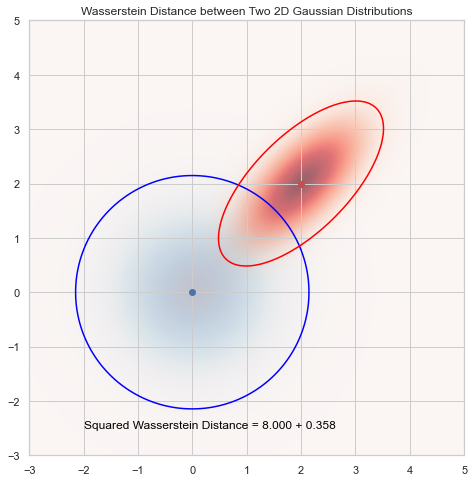
\includegraphics[width=0.5\textwidth]{images/Wasserstein.png}  
\end{center}
\end{frame}


\begin{frame}{Lifting completeness from $X$ to $\mathcal{P}_p(X)$}
    We remind ourselves of the metric version of the $L^p$ spaces. 
        $$L^p(\Omega,\mathcal{F}, P, X) \coloneqq \left\{ f : \Omega \rightarrow X \mid f \text{ measurable }, \int_\Omega d^p(f,z_0) d P < \infty \right\}$$ with$$d_{L^p}^p(f,g) \coloneqq \int_\Omega d^p(f,g) dP$$
        These are not necessarily vector spaces, but one can show that this more general notion of $L^p$ space is still complete if $(X,d)$ is. \\
        This completeness is important for the following Theorem.
    \begin{theorem}
        Let $(X,d)$ be a complete metric space, then $(\mathcal{P}_p(X), W_p)$ is complete.
    \end{theorem}
\end{frame}

\begin{frame}{Iterated Dudley Lemma}
    We want to represent a sequence of measures $(\mu_n)$ as the marginals of some measure in an infinite product space. \\ 
    \vspace{0.5cm}
    For that we need the iterated Dudley Lemma. Note that we also allow $N = \infty$ in this Lemma, in that case, the $\leq$ become $<$.
    \begin{lemma}
        Let $N \geq 3$ and for any $n \leq N$ $(X_n,d_n)$ Polish, $\mu_n \in \mathcal{P}(X_n)$ and $\theta_n \in \Gamma(\mu_{n-1},\mu_n)$. \\ 
        Then there exists $\pi_n \in \mathcal{P}(X_1\times ... \times X_n)$ for any $n \leq N$ such that.
        \begin{enumerate}
            \item $p^{1,...,n-1}_{\#} \pi_n = \pi_{n-1}$ for $2 \leq n \leq N$
            \item $p^i_{\#} \pi_n = \mu_i$ for $1 \leq i \leq n \leq N$
            \item $p^{i-1,i}_{\#} \pi_n = \theta_i$ for $2 \leq i\leq n \leq N$
        \end{enumerate}
    \end{lemma}
    Proof is just applying the Dudley Lemma iteratively (hence the name :).
\end{frame}

\begin{frame}{Prove of completeness}
    We again consider $p = 2$. Assume $(\mu_n) \subseteq \mathcal{P}_2(X)$ is Cauchy. 
    \begin{enumerate}
        \item Applying Iterated Dudley on $(X,\mu_n)$ to get $(\pi_n)_{n \in \mathbb{N}}$ 
        \item Get $\pi_\infty$ on $\mathbb{X} = \prod_{i = 1}^{\infty} X$ with $p^{(1,...,n)}_{\#}(\pi_\infty) = \pi_n.$
        \item Show that the projections $(p_n)$ are Cauchy in $L^2(\mathbb{X}, \mathcal{B}_\infty, \pi_\infty,X)$
        \item Use that $L^2(\mathbb{X}, \mathcal{B}_\infty, \pi_\infty,X)$ is complete to get $p_n \rightarrow p_\infty$
        \item Define $\mu_\infty = (p_\infty)_{\#}(\pi_\infty)$ and prove $\mu_n \xrightarrow{W_2} \mu_\infty.$
    \end{enumerate}
    \begin{reminder}
        If $\sum_{k = 1}^{\infty} d(x_n,x_{n+1}) < \infty$ then $(x_n)$ is Cauchy. \\
        \vspace{0.5cm}
        Also earlier in the Book, we had $$S_{\#}(P) = \mu \quad \text{ and } \quad T_{\#}(P) = \nu \Rightarrow (S,T)_{\#}(P) \in \Gamma(\mu,\nu).$$
    \end{reminder}
\end{frame}

\begin{frame}{Duality for the Wasserstein Distance}
    By the Kantorovich-Rubinstein Duality we have \begin{align*} W_1(\mu,\nu) &= \sup_{(\phi,\psi) \in I_c} \left\{ \int_X \phi d\mu + \int_X \psi d\nu \right\} \\ &= \sup_{\|\phi\|_{Lip} \leq 1} \left\{\int_X \phi d\mu + \int_X \phi^c d\nu  \right\} 
       \\ &= \sup_{\|\phi\|_{Lip} \leq 1} \left\{\int_X \phi d\mu - \int_X \phi d\nu  \right\} \end{align*}
       where the first equality holds for any $W_p$ distance, the latter need that $c = d$.
\end{frame}


\begin{frame}{Wasserstein distance for $p = \infty$}
    If we restrict ourselves to $\mathcal{P}_\infty(X)$, the space of probability measures with bounded support. We can also define $W_\infty$ as the limit of $W_p$.
    \begin{align*}\lim_{p \to \infty} W_p(\mu,\nu) &= W_\infty(\mu,\nu) =\text{inf}\{\|d(x,y)\|_{L^\infty}(\pi) \mid \pi \in \Gamma(\mu,\nu)\} \\
    &= \underset{\pi \in \Gamma(\mu,\nu)}{\text{inf}}\text{inf}\{C \geq 0 \mid |d(x,y)| \leq C \text{ for } \pi \text{ almost all } (x,y)\} \end{align*} 
    and we have $$(\mathcal{P}_\infty(X), W_\infty) \text{ is a metric space}$$ 
\end{frame}



%%%%%%%%%%%%%%%%%% End of Presentation %%%%%%%%%%%%%%%%%


\end{document}